% !TEX root = ../main.tex

\section{Introduction} \label{sec:introduction}

Detecting structural break points is an essential tool in analyzing time series.
Structural break points are points on a time series where the pattern of the
time series measurements changes in the amplitude. A simple example is shown in
figure~\ref{fig:simple-graph} where the break point is easily detected at $t =
500$. Structural breaks are where the pattern of a time series changes. 

In the example above, the break point is easy to detect. As usual, the
real world is far more messy. In figure~\ref{fig:covid19-dk-en},
which shows the number of patients hospitalized in Denmark due to Covid19, the
break points are less obvious. This is where detecting break points is
important: Being able to recognize when the pattern changes, so that a pandemic
does not run amok or looking for fluctuations in the stock market. \todo{Please
find another example than the stock market}

In this project, the break points are found by using a so-called genetic
algorithm. This algorithm mimics natural evolution: A number of individuals
(solutions that indicate the positions of break points) mutate and mate during
generations where survival of the fittest is the rule. In the end, the best
solution will (hopefully) have found all the break points. 

This project will focus on implementing the algorithm in the programming
language Java and make a simple application. The application will give the user
the ability to tweak some of the algorithm's parameters and see the break points
directly on the time series graph. Further improvements to the speed of the algorithm
will also be implemented "under the hood". 

\todo{Make the left figure more pretty!}

\begin{figure}[h]
    \centering
    \begin{subfigure}[b]{0.48\textwidth}
        \centering
        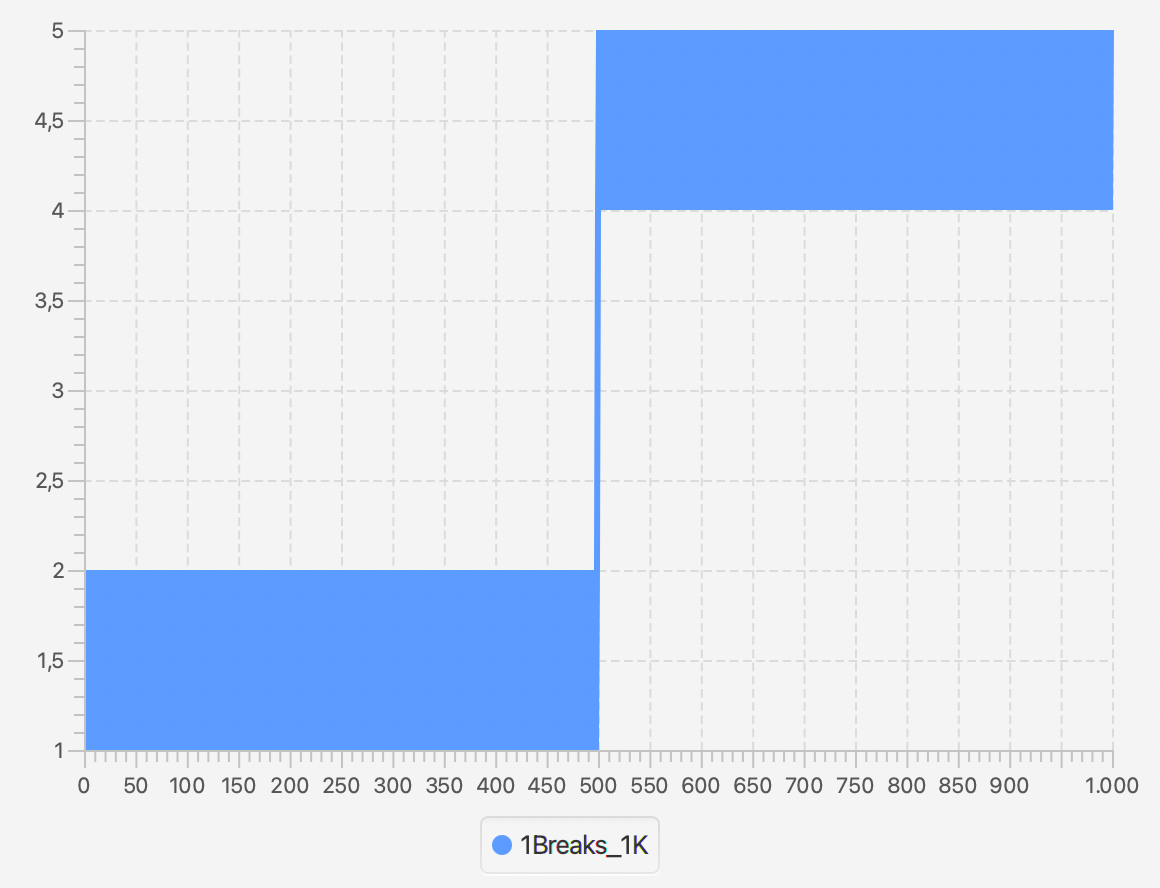
\includegraphics[width=\textwidth]{fig/simple-graph.png}
        \caption{Graph with break point at $t = 500$}
        \label{fig:simple-graph}
    \end{subfigure}
    \hfill
    \begin{subfigure}[b]{0.48\textwidth}
        \centering
        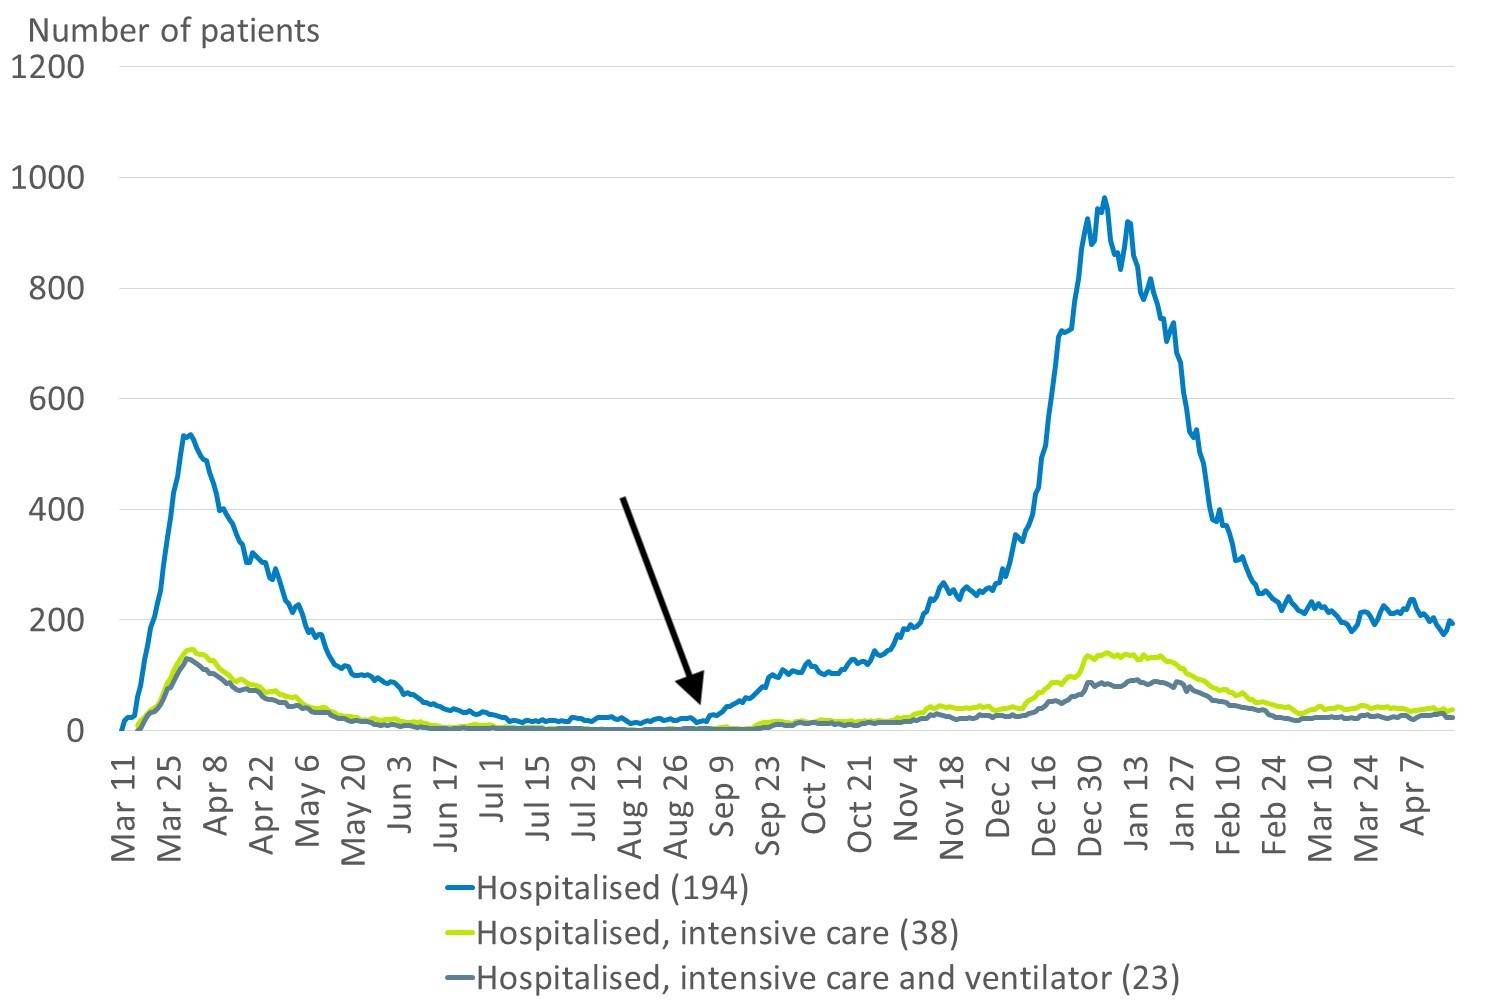
\includegraphics[width=\textwidth]{fig/covid19-dk-en.jpg}
        \caption{Source: The Danish Regions}
        \label{fig:covid19-dk-en}
    \end{subfigure}
    \caption{Two figures illustrating break points in time series}
    \label{fig:intro-figure}
\end{figure}